\section{Trening własnej kaskady (Maciej Plewka)}

W celu zrealizowania detekcji naszej karty, potrzebne było wytrenowanie własnej kaskady klasyfikatorów Haar'a. W tym celu skorzystano z aplikacji dostarczonych przez openCV szerzej opisanych w rozdziale \ref{sec:opencv}. Cały proces uczenia został wykonany na komputerze osobistym z procesorem Intel Core i3 4000M o częstotliwości taktowania zegara 2,4 GHz i 8GB pamięci operacyjnej. Biblioteka OpenCV wraz z aplikacjami zostały skompilowane ze źródeł znajdujących się w publicznym repozytorium \cite{OpenCVSource}. Dodatkowo podczas budowania biblioteki zaznaczono flagę by zostało włączone wspieranie standardu OpenCL, który umożliwia zrównoleglenie obliczeń, co znacząco przyspiesza czas działania zbudowanych aplikacji.

\subsection{Zbiór danych uczących}

Zdobycie przynajmniej 2000 zdjęć wykorzystanych do uczenia jest dużym problemem. Dlatego dane uczące zostały wygenerowane przy użyciu aplikacji opencv\_createsamples, opisanej w rozdziale \ref{sec:generowanieZdjec}. Do wygenerowania zdjęć pozytywnych wykorzystano 5 zdjęć na których znajduje się tylko i wyłącznie nasz wzór. W pierwotnych założeniach rozpoznawany miał być rewers wybranej karty. Z powodu skomplikowanego wzoru rewersu karty, gdzie kolor biały i czarny gęsto się przeplata, postanowiono proces treningu przeprowadzić także na własnej, przygotowanej karcie, której wzór jest stosunkowo prosty. Potrzebny był także zbiór zdjęć na którym nie znajduje się nasza karta. Wykorzystano do tego serwis internetowy \cite{imageNetOrg}, który posiada bogaty zbiór sklasyfikowanych zdjęć, udostępniony z intencją wykorzystania do uczenia maszynowego. Z tej bazy zdjęć pobrano niecałe 3000 zdjęć sklasyfikowanych jako niedźwiedzie, robaki, gitary, pociągi i książki. Zbiór tych zdjęć pogrupowano na 5 podgrup po 500 zdjęć. W celu skrócenia czasu treningu zdjęcia te zostały zmniejszone za pomocą funkcji resize biblioteki openCv, która wykorzystuje interpolację. Jest to proces który dzięki któremu wyznaczamy wartość nowego piksela na podstawie innych sąsiadujących z nim pikseli. Zdjęcia tła zostały zmniejszone do rozdzielczości 120x186 pikseli. Jest to wymiar którego stosunek wysokości i szerokości jest taki sam jak w przypadku karty. Obrazy wzorów kart zostały również pomniejszone, jednak do rozdzielczości 40x62. Z początku rozważano użycie mniejszego rozmiaru zdjęć, co spowodowałoby zmniejszenie liczby możliwych cech Haar'a dla obiektu. Dość skomplikowany wzór awersu karty powodował nieczytelność zdjęcia, a co za tym idzie cechy słabo generalizowały by odpowiednie fragmenty prawdziwego obiektu. Wszystkie wykonane operacje dla obu wzorów dalej będą wykonywane analogiczne, z tymi samymi parametrami.

\begin{figure}[H]
	\centering
	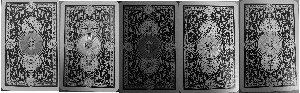
\includegraphics[scale=1.0]{imgs/RewersyKarty.jpg}
	\caption{Rewersy kart użyte do treningu}
	\label{fig:KartaRewers}
\end{figure}
.

\begin{figure}[H]
	\centering
	
\includegraphics[scale=1.2]{imgs/Karta?.jpg}
	\caption{Wzory własnej karty użyte do treningu}
	\label{fig:KartaTajemnicza}
\end{figure}

Zdjęcia zostały podzielone na 5 katalogów, by każdy z nich odpowiadał jednemu obrazowi wzoru. Do utworzenia zbioru zdjęć pozytywnych potrzebujemy jeszcze pliku tekstowego w którym wylistowane będą ścieżki do zdjęć będących tłem wybranego wzoru. Posiadając wszystkie wymagane pliki tj. zdjęcie z pozytywnym wzorem oraz plik tekstowy ze ścieżkami do obrazów tła, możemy uruchomić aplikację opencv\_createsamples. Dodatkowo ustawiono losowy kąty nachylenia na, do 0,2 rad w płaszczyźnie x oraz y natomiast w płaszczyźnie z do 0,1 rad. Koniecznym też było ustawienie odpowiedniego koloru tła naszego pozytywnego zdjęcia. Nasze pozytywne zdjęcia zawierają tylko i wyłącznie przycięty wzór, bez żadnego tła. Domyślnie jako kolor tła jest brana wartość 0 tj. kolor czarny, co w przypadku obu kart powoduje ignorowanie niektórych fragmentów, powodując że są one jakby przezroczyste. Kolor tła w tej aplikacji określany jest jako zakres obliczany z wartości parametrów bgcolor oraz bgthresh. Jako tło brany jest każdy kolor z przedziału od bgcolor-bgthresh do bgcolor+bgthresh. W naszych wzorach tło nie występowało, więc jako parametr -bgcolor podano 200 tj. kolor nie znajdujący się na naszym wzorze a -bgtresh przyjęto wartość 1. Po uruchomieniu aplikacji posiadamy 2500 sklasyfikowanych zdjęć pozytywnych na których znajdują się wzory, których detekcje chcemy osiągnąć. Teraz dla każdego pliku info z informacjami na temat wygenerowanych obrazów możemy wygenerować plik z rozszerzeniem vec, który jest potrzebny do poprawnego uruchomienia aplikacji trenującej kaskadę klasyfikatorów.
Polecenie które uruchomiło wygenerowanie obrazów dla jednego pozytywnego zdjęcia i 500 zdjęć będących tłem wygląda następująco:
\begin{lstlisting}
opencv\_createsamples -img pos?/pos5.jpg -bg bg5.txt -info info/info5.list -pngoutput info/ -bgcolor 200 -bgthresh 1 -maxxangle 0.2 -maxyangle 0.2 -maxzangle 0.1 -num 500 -w 40 -h 62
\end{lstlisting}


Aplikacja została uruchomiona dla pięciu różnych zdjęć karty. Kolejne polecenia uruchamiające różniły się wskazaniem na inne zdjęcie wzorca, inny plik ze ścieżkami zdjęć będących tłem oraz innym plikiem info do którego zapisywane są informacje o wygenerowanych zdjęciach.
Ostatnim krokiem kończącym proces przygotowania danych jest połączenie pięciu plików vec w jeden, który będzie jednym z argumentów wejścia programu opencv\_traincasscade. Wykorzystujemy do tego skrypt mergevec.py \cite{mergeVec}. Narzędzie to przyjmuje dwa argumenty:
\begin{itemize}
	\item -v \textless Scieżka do katalogu z plikami vec które należy scalić \textgreater
	\item -o \textless nazwa scalonego wynikowego pliku \textgreater
\end{itemize}
Pliki vec skopiowano do katalogu vec, skrypt mergevec.py znajduje się w katalogu mergevec. Polecenie które wygenerowało scalony plik vec wygląda następująco: 
\begin{lstlisting}
python mergevec/mergevec.py -v vec/ -o posss.vec
\end{lstlisting}
\subsection{Proces treningu}

Proces treningu kaskady przeprowadzono dla dwóch wzorów. Jednym z nich jest rewers karty, z talii kart do gier karcianych, drugi to przygotowany przez nas wzór przedstawiający znak zapytania na czerwonym tle. Dla każdego wzorca proces uczenia odbywał się na podstawie zdjęć wygenerowanych i przeskalowanych to tej samej wielkości. Początkowo zakładano by rozmiar wzorców wynosił 20x31 pikseli, by obniżyć do minimum liczbę możliwych cech Haar'a.
Po przeskalowaniu zdjęć do określonej wielkości okazało się, że rewers kart jest bardzo niewyraźny, co ogranicza zdolność cech do generalizowania. Dlatego rozmiar wzorców ustalono na 40x62 pikseli. Wymiar ten zachowuje proporcje naszych kart. Liczba unikalnych cech Haar'a dla takiego rozmiaru wynosi 2978000. Rysunki \ref{fig:KartaTajemnicza} i \ref{fig:KartaRewers} przedstawiają wzory użyte do treningu kaskad po przeskalowaniu. Przeprowadzony trening odbywał się na zbiorze tysiąca ośmiuset zdjęć pozytywnych oraz dziewięciuset zdjęciach negatywnych. Obrazy te posiadały jednakowy rozmiar 120x186. Zastosowano taki rozmiar by skrócić czas treningu, ponieważ dla większego zdjęcia podczas treningu trzeba przeanalizować większą ilość fragmentów. W celu zapobiegnięcia przeuczeniu tj. sytuacji w której kaskada będzie wytrenowana tylko i wyłącznie do rozpoznawania zdjęć treningowych, postanowiono ograniczyć się do wygenerowania dwunastu etapów kaskady. Do uruchomienia aplikacji potrzebne są: wygenerowany plik vec oraz plik ze ścieżkami zdjęć negatywnych. Współczynniki pozytywnych decyzji i negatywnych zostały zastosowane takie jak domyślne wartości aplikacji TPR = 0.995 a FPR = 0.5. Komenda uruchamiająca trening dla obu wzorów wygląda następująco:

\begin{lstlisting}
opencv\_traincascade -data data -vec posss.vec -bg bgall.txt -numPos 1800 -numNeg 900 -numStages 11 -w 40 -h 62
\end{lstlisting}

\subsubsection{Trening detercji rewersu karty}

Ze względu na pierwotne założenia pierwszym wzorem na którym był przeprowadzony proces detekcji był rewers karty. Proces uczenia trwał trzydzieści osiem godzin. Wytrenowana kaskada składa się z dwunastu etapów i posiada dziewięćdziesiąt osiem cech opisujących wzór karty.

\begin{figure}[H]
	\centering
	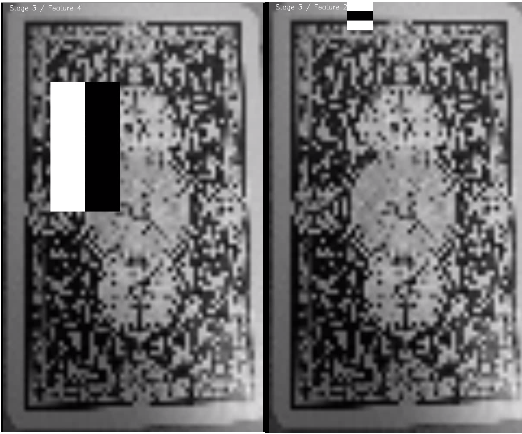
\includegraphics[scale=0.2]{imgs/cechyRewers.png}
	\caption{Cechy opisujące rewers karty}
	\label{fig:cechyRewers}
\end{figure}

Rysunek \ref{fig:cechyRewers} przedstawia przykładowe cechy włączone do kaskady celnie opisuje wzór. Wytrenowana kaskada słabo radzi sobie z jednoznaczną detekcją obiektów. Na dziesięć zdjęć na których znajduje się tylko i wyłącznie karta na różnych tłach, tylko na dwóch z nich celnie odnaleziono obiekt. Dodatkowo w obrębie karty odnalazł także kilka obiektów, więc na żadnym ze zdjęć nie był w stanie jednoznacznie wskazać obiektu. Powodem takiego wyniku jest najprawdopodobniej skomplikowany wzór, który gęsto przeplata biały i czarny kolor. Spowodowało to, że cechy pasują do różnych miejsc w obrębie karty, przez co nie jest w stanie jednoznacznie odnaleźć obiektu. Kolejnym elementem wpływającym niekorzystnie na detekcję jest pomniejszony obraz wzoru. Spowodowało to, że cechy odzwierciedlają wyraźnie zniekształconą wersję obiektu.

\subsubsection{Trening detekcji karty ze znakiem zapytania}

Z powodu słabej skuteczności kaskady przeznaczonej do detekcji rewersu karty postanowiono użyć innego wzoru. Słaba skuteczność spowodowana była najprawdopodobniej skomplikowanym wzorem. Trening kaskady został uruchomiony z takimi samymi parametrami jak w przypadku rewersu karty. Cały proces uczenia zajął jedenaście godzin. Kaskada składa się z jedenastu etapów, ponieważ po jedenastym etapie, współczynnik FPR osiągnął już zadowalający poziom. Kaskada składa się z pięćdziesięciu czterech cech Haar'a.

\begin{figure}[H]
	\centering
	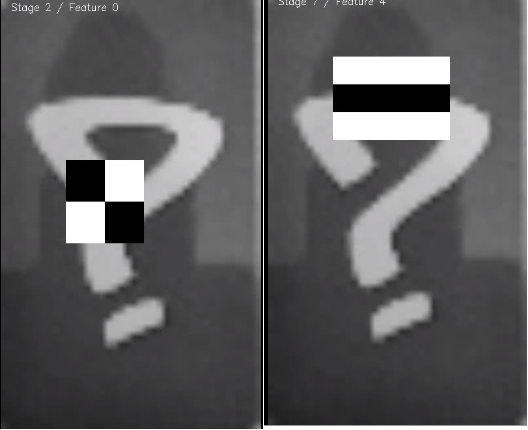
\includegraphics[scale=0.2]{imgs/cechy?.png}
	\caption{Cechy opisujące naszą kartę}
	\label{fig:cechy?}
\end{figure}

Rysunek \ref{fig:cechy?} przedstawia przykładowe cechy celnie opisujące naszą kartę. Na dziesięć zdjęć zawierających jeden obiekt na jednolitym tle, obiekt został poprawnie oznaczony w każdym z nich. Trzeba zaznaczyć, że na trzech zdjęciach zaznaczone zostały także fragmenty niezwiązane z szukaną kartą. Otrzymano zatem siedem jednoznacznych decyzji o odnalezieniu obiektu, więc można powiedzieć, że osiągnięto sukces.
